here are files for the mathematical style Im using, I will alter update text based on them 



\section{Observational Study Domains} \label{sec:obs_domains}



Depending on the dynamic interactions among biomass, climate, and human activity, each region of interest observed by the satellite could exhibit a characterizable fire intensity over a temporal pattern; in other words, each region of interest could have a specific fire season. With this in mind, the satellite constellation mission modeled in this work shall have as a requirement an observational temporal window synchronized with these fire season periods. Therefore, the spacecraft architecture shall be analyzed against\textit{ Fire-Prone Regions (FPR)}, or piroregions, here defined as the \textit{Core Study Domain ($\mathcal{D}_{core}$)} and the \textit{Generalized Study Domain ($\mathcal{D}_{general}$)}. Both of these objects are composed of subsets of \textit{Regions of Interest (ROI)} which are defined in a spatial $\mathcal{R}$ and temporal $\mathcal{T}$ coordinate domains. Therefore, each ROI can contain flammable biomass that may exhibit distinct fire dynamics over time, leading to a temporal spread of \textit{Fire Activity (FA)} in these domains. 



\subsubsection{Formal Definition of Study Domains}\label{sec:formal_def_domains}



To ensure the satellite constellation meets precise operational requirements, we define the mission environment as a four-dimensional manifold $\mathcal{M}$ (Space-Time). Since the satellite orbit is governed by orbital mechanics while the observation targets are subject to planetary dynamic motion, we must rigorously define the relationship between the inertial and rotating frames.



We establish the base reference frame of $\mathcal{M}$ as the \textbf{Earth Mean Equator and Equinox of J2000 (EME2000)}, hereafter denoted as the Inertial Frame $\mathcal{F}_{J2000}$ (corresponding to the IJK system in Fig. \ref{fig:vallado_ijk_frame}). However, the regions of interest for the constellation are fixed to the rotating Earth. Therefore, we define the boundaries of the study domains relative to the \textbf{World Geodesic System 84 (WGS84)}, which has an Earth-Centered Earth-Fixed (ECEF) frame, hereafter denoted as the Earth Frame $\mathcal{F}_{\oplus}$, \inlineReq{R9}.

\begin{figure}[H]

    \centering

    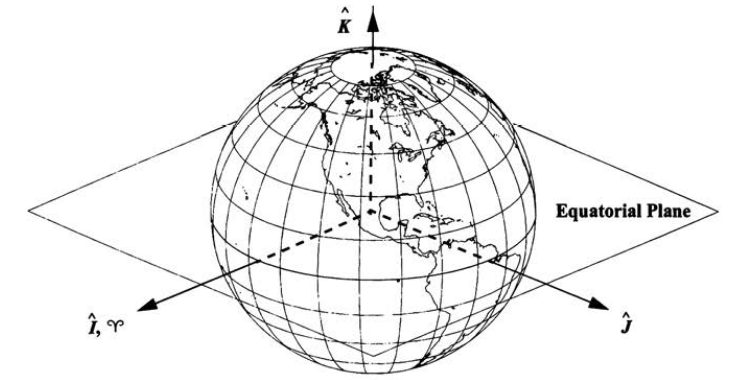
\includegraphics[width=0.65\linewidth]{images/Geocentric_Equatorial_System_(IJK)_F_earth.png}

    \caption{The Geocentric Equatorial Coordinate System (IJK) as defined by Vallado \cite{mcclain2001fundamentals}. The frame is defined by Earth's origin, the equatorial plane, and the vector $\hat{I}$ pointing toward the Vernal Equinox ($\Upsilon$). In this thesis, the IJF frame system represents the Inertial Frame $\mathcal{F}_{J2000}$ used for orbit propagation. It is distinct from the rotating Earth Frame $\mathcal{F}_{\oplus}$ (ECEF), which holds the study Domain $\mathcal{D}$ that rotates with the Earth.}

    \label{fig:vallado_ijk_frame}

\end{figure}

Formally, the universal manifold $\mathcal{M}$ is defined as the Cartesian product of spatial and temporal domains, mathematically expressed as:



\begin{equation}

    \mathcal{M} = \mathbb{E}^3 \times \mathcal{T} \cong \{ (P, t) \}

    \label{eq:manifold}

\end{equation}



Here, $\mathbb{E}^3$ denotes the 3-dimensional spatial Euclidean Space, while $\mathcal{T}$ represents the absolute time continuum expressed in Coordinated Universal Time (UTC) . The relation $\mathcal{T} \cong \mathbb{R}$ establishes the structure-preserving mapping, or isomorphism, between physical time and the real number line, ordered by the epoch $t$. Consequently, any unique event in the manifold is represented by the pair $(P, t)$, where $P \in \mathbb{E}^3$ is a spatial point and $t \in \mathcal{T}$ is a temporal moment.



To enable orbital analysis within this manifold $\mathcal{M}$ , we define an origin $O$ at the Earth's Center of Mass. This definition permits the mapping of any spatial point $P$ to a position vector $\mathbf{r}$ in the inertial frame $\mathcal{F}_{J2000}$ via the transformation $\mathbf{r} = P - O$.



A Study Domain $\mathcal{D} \subset \mathcal{M}$ is defined as the subset of inertial points occupied by a specific geographic region of interest $ROI_{\text{W84}}$ during a specific temporal fire season window $\mathcal{T}_{fire}$. Mathematically, this domain is expressed as:

\begin{equation}

    \mathcal{D} = \{ (\mathbf{r}_{J2000}, t) \in \mathcal{M} \mid \mathbf{r}_{J2000} = \mathbf{T}_{\oplus \to J2000}(t) \cdot \mathbf{r}_{\oplus}(\phi, \lambda, h), \ t \in \mathcal{T}_{fire} \}

\end{equation}

In this formulation  $\mathbf{r}_{\oplus}(\phi, \lambda, h)$ denotes the position vector in the Earth Frame $\mathcal{F}_{\oplus}$, derived from the geodetic coordinates of latitude $\phi$, longitude $\lambda$, and altitude $h$. The target observation fire season is represented by $\mathcal{T}_{fire} = [t_{start}, t_{end}]$ in UTC. $\mathbf{T}_{\oplus \to J2000}(t)$ is the time-dependent coordinate transformation. This operator accounts for Earth’s rotation, precession, and nutation, projecting the fixed ground coordinates from $\mathcal{F}_{\oplus}$ into the inertial frame $\mathcal{F}_{J2000}$.  



This process of coordinate transfers of study domain $\mathcal{D}$ rotating on Earth's frame to an inertial frame allows calculations connecting $\mathcal{D}$ with the satellite propagation, making possible knowledge such coverage time, revisits, communication links, satellite imagery retrieval from datasets, etc.



Using this study domain formalism, we define the two primary objects of this study:

\begin{itemize}

    \item \textbf{Core Study Domain ($\mathcal{D}_{core}$)}: The subset of $\mathcal{M}$ constrained by the geographical boundaries of Mainland Portugal and the temporal bounds of its fire season\inlineReq{R10}.

    \item \textbf{Global Study Domain ($\mathcal{D}_{global}$)}: The subset of  $\mathcal{M}$  containing Earth's fire-prone regions each with a specific temporal fire activity \inlineReq{R11}.

\end{itemize}



\subsection{Core Study Domain}



This section details the properties of $\mathcal{D}_{core}$, establishing its spatial region elements $\mathcal{R}_{core}$ and core temporal boundaries $\mathcal{T}_{core}$ for the definition of the mission over mainland Portugal. Formally, the domain is defined as the Cartesian product of these spatial and temporal sets:

\begin{equation}

    \mathcal{D}_{core} = \mathcal{R}_{core} \times \mathcal{T}_{core} \subset \mathcal{M}

\end{equation}

This definition is useful for analysis, such as observation events that require the satellite state vector or field of view to coincide with points $p \in \mathcal{R}_{core}$ at a time $t \in \mathcal{T}_{core}$. 



\subsubsection{Core Spatial Elements}



The spatial component $R_{core}$ is composed of a set of geometrical objects defined on the reference ellipsoid of the WGS84 system. We categorize these objects into two topological types:



\begin{enumerate}

    \item \textbf{Point Target (P):} Defined as a single vertex coordinate $P(\phi, \lambda, h)$, representing a point with zero-dimensional location of interest (e.g., a ground target, specific ground station, or a city location).



    \item \textbf{Region Target ($\mathcal{R}$):} Defined as the union of $M$ distinct surface patches $S_j$. Mathematically, the region target is a multi-polygon defining a compact region $\mathcal{R} = \bigcup_{j=1}^{M} S_j$. Each patch $S_j$ is a surface bounded by a closed geodesic polygon. The boundary of such a polygon $S_j$, denoted as $\partial S_j$, is a piecewise geodesic curve consisting of connected geodesic segments defined by an ordered set of $N_j$ vertices $\{P_{i}\}_{i=1}^{N_j} = \{P_{1}, P_{2}, ..., P_{N_{j}}\}$, where the boundary is closed by the segment $P_{N_{j}}$ to $P_{1}$.

\end{enumerate}



\begin{figure}[ht]

  \centering

  \fbox{%

    \begin{minipage}[c][1cm][c]{0.9\linewidth}

      \centering \textit{[Figure placeholder: Diagram: Point Target P vs. Region Target $\mathcal{R}$ defined by Geodesic Boundary]}

    \end{minipage}%

  }

  \caption{Topological definition of Point and Region targets on the WGS84 Ellipsoid.}

  \label{fig:drawing_core_spatial_elements}

\end{figure}



\subparagraph{Application to Mainland Portugal ($\mathcal{R}_{pt}$)}\hspace{0pt}



Applying these definitions, the spatial region of mainland Portugal is modeled as a Region Target $\mathcal{R}_{pt}, \inlineReq{R12}$. 

Its boundary, $\partial \mathcal{R}_{pt}$, is established using standard geospatial vector data formats, specifically ESRI Shapefiles (.shp) or GeoJSON. \footnote{These files encode the set of vertex coordinates $\{P_{i}\}_{i=1}^{N_j}$ in the Coordinate Reference System (CRS) EPSG:4326 (WGS84 Latitude/Longitude). For the computational simulation, these geometries are processed using standard Python geospatial modules, such as \texttt{geopandas} for data management and \texttt{shapely} for geometric operations (e.g., point-in-polygon verification, coverage maps).}

At figure \ref{fig:map_D_core_elements}, $\mathcal{R}_{pt}$ can be visualized.





\subparagraph{Application to points inside Portugal ($\mathcal{P}_{pt}$)}\hspace{0pt}

 

It is interesting to define point targets $P_i$ within Portugal's $\mathcal{R}_{pt}$ boundaries to verify the local performance of the satellite constellation, such as the revisit time over a city or fire-prone location. 

To decide which points to choose, we perform the following verification. One can analyze studies of burned area (Fig \ref{fig:map_BA_global_decrease_1998_2015}, Fig \ref{fig:BA_global_decade_fire_seasons}) and fire activity (Fig.\ref{fig:fire_season_types}  to  Fig. \ref{fig:fire_season_start2_end2}). The combination of this kind of multivariate study can lead to the production of a global map of fire-climate classes stratified by the intensity of each fire-prone region, as done by Senande-Rivera et al., reproduced here in Fig  \ref{fig:fire_prone_global_now_future}-b \cite{senande-rivera_spatial_2022}. 



As seen in Rivera's work, Portugal and most of the Iberian Peninsula have a fire-climate class defined as Temperate-dry hot season (Te-dhs), with recurrent (r) fire-prone regions quantified by more than seven intense fires per decade. More specifically, this zone is defined as Te-dhs-r (Temperate-dry hot season-recurrent) (TODO:-connects this to the global part- and is spread almost symmetrically over the equator line happening on latitudes $\approx 40º \pm 5º$). Because this peninsular area exhibits almost homogeneous fire dynamics, the best strategy to achieve optimal constellation coverage is to select a point target centralized in Portugal. As we wish this point to be revisited often by the satellite constellation, this central point is named $P_{revisit}$.

Therefore, this work selects Coimbra as the main target to revisit inside the core study domain because it is the largest city, approximately in the center of Portugal, and surrounded by fire-prone regions \inlineReq{R13}. 

\begin{equation}

    P_{revisit} = P_{Coimbra}

\end{equation}





To verify the satellite constellation performance in other relevant Portuguese i points $\mathcal{P}_{pt,i}(\phi, \lambda, h)$, the table \ref{tab:pt_coords} with geographical references will be used during the simulation\inlineReq{R14}. This points are visualized in the map \ref{fig:map_D_core_elements}.



\begin{table}[ht]

\centering

\caption{Point target coordinates $\mathcal{P}_{pt,i}(\phi, \lambda, h)$ of selected regions of interest inside the Portugal mainland region target $\mathcal{R}_{pt}$ which is contained in the core study domain $\mathcal{D}_{core}$. (WGS84). (TODO: Recheck these values in GEE or geopandas)}

\label{tab:pt_coords



\subsubsection{Core Temporal Boundaries}



With the core spatial region $\mathcal{R}_{core}$ established for Mainland Portugal, $\mathcal{R}_{core} \equiv \mathcal{R}_{pt}$, the core study domain now requires a observational window here, represented as a temporal set $\mathcal{T}_{core}\subset\mathcal{T}$ describing the  fire season expected to occur and for which the satellite constellation shall have the performance assessed.



 We establish the full year of 2024 as the simulation core temporal  \inlineReq{R15}. Formally, $\mathcal{T}_{core}$ is defined as the continuous interval:

\begin{equation}

    \mathcal{T}_{core} = [t_{start_{2024}}, t_{end_{2024}}] \subset \mathcal{T}

\end{equation}

Where $t_{start_{2024}}$ corresponds to 2024-01-01 00:00:00 UTC and $t_{end_{2024}}$ to 2024-12-31 23:59:59 UTC.



\subparagraph{Portugal season markers}\hspace{0pt}



\subparagraph{Critical observational reference for the constellation}\hspace{0pt}



Portugal's fire season starts in March, with increasing fire activity peaking in summer. This is the critical observation period for the constellation, which has two main intense peaks in the first week of August and around the third week. The constellation shall have the best coverage in this month, with August 18 as the main fire peak reference \inlineReq{R16}. 

\begin{equation}

    t_{\text{peak fire ref}} = \text{ August 18th }

    \label{eq:peak_fire_ref_day}

\end{equation}

After this period of faster pyrodynamics, the season extends with decreasing intensity until fading in February of the next year. 



\subsection{Generalized Study Domain}



This section details the properties of the Global Study Domain $\mathcal{D}_{global}$, establishing its spatial region elements $\mathcal{R}_{global}$ and temporal boundaries $\mathcal{T}_{global}$. Formally, the domain is defined as the Cartesian product of these sets:

\begin{equation}

    \mathcal{D}_{global} = \mathcal{R}_{global} \times \mathcal{T}_{global} \subset \mathcal{M}

\end{equation}



\subsubsection{Global Spatial Element}



To construct the global spatial definition, we extend the previous topological concepts of the Core Domain. However, unlike $\mathcal{R}_{core}$, which is bounded by static geopolitical borders (Mainland Portugal), the global region $\mathcal{R}_{global}$ is defined by phenomenological boundaries, specifically, the probability of fire occurrence on different types of biomass and climate \inlineReq{R17}.



We designate this spatial object as the Earth's Fire-Prone Region Target\textbf{ $\mathcal{R}_{\oplus_{FPR}}$}. Mathematically, it is defined not as a single contiguous shape, but as the union of all disjoint surface patches $S_k$ on the planetary ellipsoid that have fire-prone characteristics:



\begin{equation}

    \mathcal{R}_{global} \equiv \mathcal{R}_{\oplus_{FPR}} = \bigcup_{k} S_k  \mid  \text{Class}(S_k) \in \mathcal{C}_{fire}

\end{equation}

Where $\mathcal{C}_{fire}$ represents the set of valid fire-prone regions classifications.



\paragraph{Earth's Fire-Prone Regions Targets ($\mathcal{R}_{\oplus_{FPR}}$)} \hspace{0pt}



The boundaries of these surface $S_k$ are determined by the fire-climate classes derived from historical satellite data (as seen in Fig. \ref{fig:fire_prone_global_now_future}), methodology proposed by Senande-Rivera et al. \cite{senande-rivera_spatial_2022}. Consequently, $\mathcal{R}_{\oplus_{FPR}}$ acts as a spatial filter, restricting the mission analysis to relevant latitudes and ecosystems (e.g., Mediterranean, Savanna, Temperate) while excluding non-flammable regions (e.g., rainy regions, deserts, oceans, ice sheets). 



\begin{figure}[H]

    \centering

    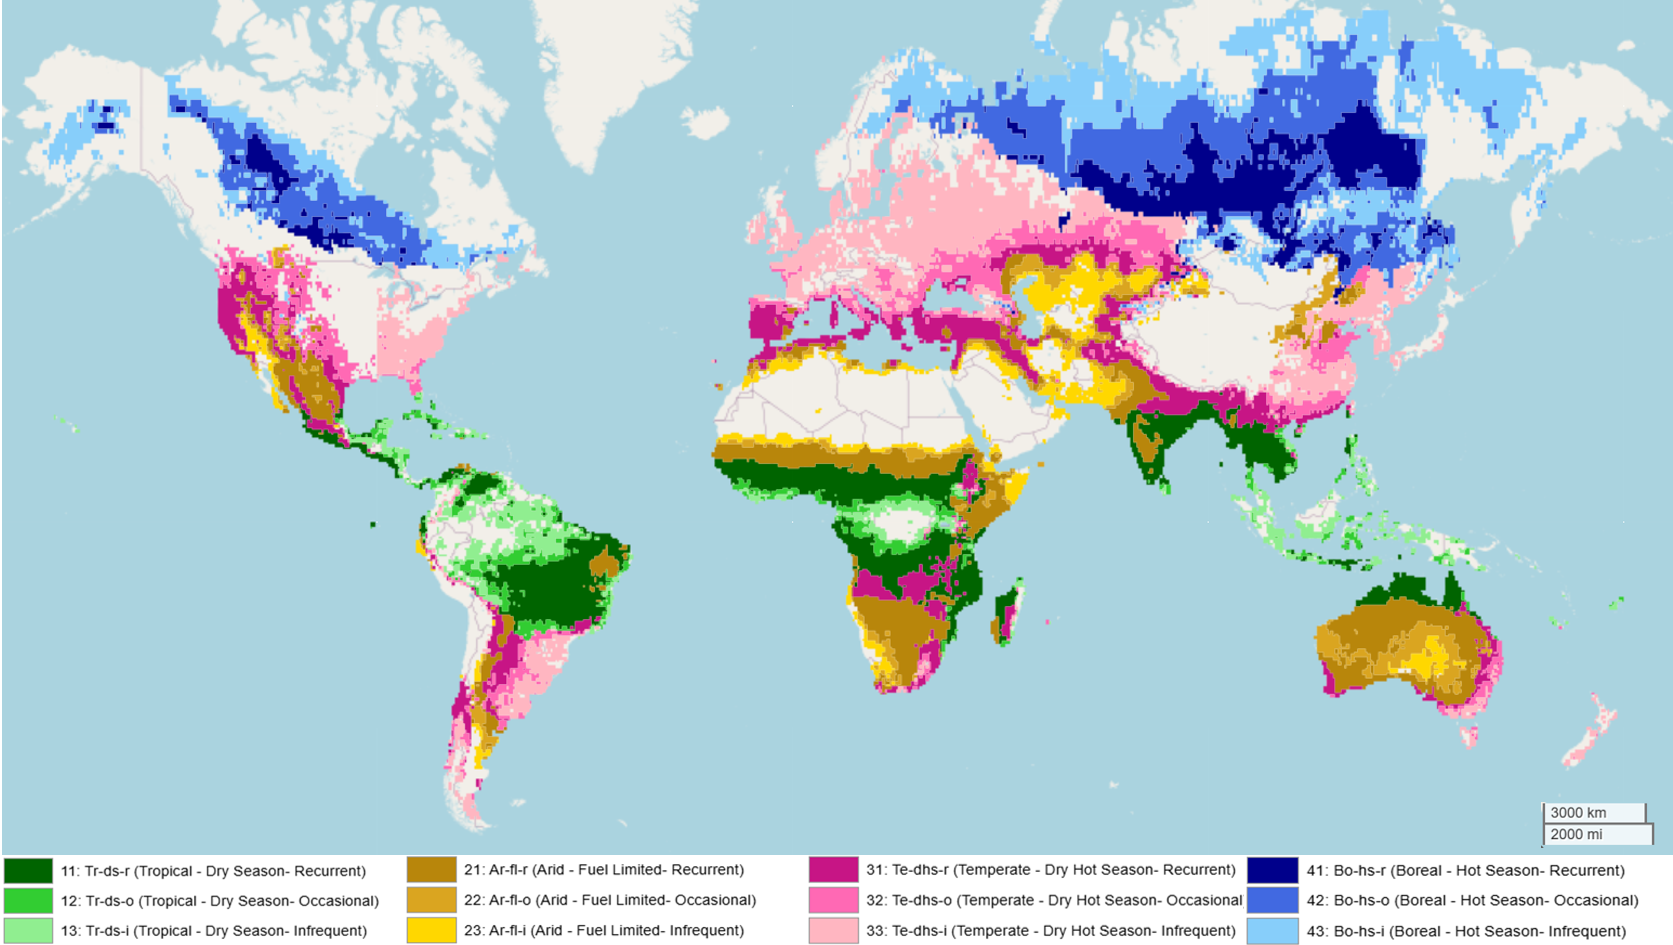
\includegraphics[width=1\linewidth]{images/map_earths_fireprone_region_targets.png}

    

    \caption{\footnotesize{\textbf{Spatial definition of the Earth's Fire-Prone Regions Target ($\mathcal{R}_{\oplus_{FPR}}$).} 

    The map visualizes the spatial element of the generalized study domain $\mathcal{R}_{global}$ as the union of all surface patches $S_k$ exhibiting valid fire-prone characteristics. Data is reconstructed from the \texttt{FC.nc} dataset provided by Senande-Rivera et al. \cite{senande-rivera_spatial_2022, senanderivera_fireclimate_2022}. The color coding corresponds to the specific fire-climate regimes $\alpha$ (e.g., \textit{Te-dhs-r}) defined in the taxonomy, stratified by climate (Tropical - Dry Season, Arid - Fuel Limited, Temperate - Dry Hot Season, Boreal - Hot Season), and fire frequency (Recurrent, Occasional, Infrequent). This spatial mask serves as the spatial operational filter for the constellation's global coverage analysis.}}

    

    \label{fig:map_earths_fire_prone_region_targets}

\end{figure}



\subparagraph{Classification Taxonomy}\hspace{0pt}



The classification assigns a descriptor to each region based on the nomenclature \texttt{[Climate]-[Type]-[Frequency]}.

First, regions are categorized into four primary climate regimes [Tropical, Arid, Temperate, Boreal] based on the Köppen–Geiger criteria. Then, specific fire thresholds are applied to identify the dominant phenomenological driver of fire activity (e.g., limited fuel vs. dry season). The intersection of these climatic and fire conditions defines the four primary classes presented bellow:



\begin{itemize}

    \item \textbf{Tr-ds (Tropical - Dry Season):} Regions driven by distinct dry seasons in tropical latitudes (e.g., Savannas).

    \item \textbf{Ar-fl (Arid - Fuel Limited):} Regions where fire activity is rare and constrained by available biomass rather than weather conditions.

    \item \textbf{Te-dhs (Temperate - Dry Hot Season):} Regions characterized by hot, dry summers (e.g., Mediterranean, Portugal). This is the primary analog to the Core Study Domain.

    \item \textbf{Bo-hs (Boreal - Hot Season):}High-latitude regions where fire activity is driven by seasonal heat waves and snow-melt timing.

\end{itemize}





\subparagraph{Frequency (Intensity)} \hspace{0pt}



Crucially for the satellite mission design of a fast wildfire constellation is the knoledge of the regions with higher frequency of fire. To assist on this goal, each climatic class is subdivided by intensity, defined by the number of \textit{Fire Prone Years (FPY)} per decade. This creates a hierarchy of observation priority:



\begin{enumerate}

    \item \textbf{Recurrent (r):} Regions with $> 7 FPY$/decade. These are high-priority targets requiring consistent monitoring if the coverage allows it depeding on the latitude.

    \item \textbf{Occasional (o):} Regions with $3 < FPY\text{/decade} \leq 7$.

    \item \textbf{Infrequent (i):} Regions with $0 < FPY\text{/decade} \leq 3$.

\end{enumerate}



\subparagraph{Operational Definition of the Global Target} \hspace{0pt}



For the purpose of this mission simulation, the generalized study domain $\mathcal{R}_{global}$ extends to all fire frequency subclasses, Recurrent (r), Occasional (o), Infrequent (i), as these represent locations where a dedicated constellation adds significant value for recurrent and intense fires, and also enables monitoring of sensitive regions, such as deforestation fronts, preservation areas, where fire activity is not yet as frequent \inlineReq{R18}.

Therefore, the valid set of target classes is defined as:

\begin{equation}

    \mathcal{C}_{fire} = \{ \text{Tr-ds}, \text{Ar-fl}, \text{Te-dhs}, \text{Bo-hs} \} \times \{ r, o, i \}

\end{equation}

This targets were modeled by Senande-Rivera et al. and they made the file of the fire-climate classification available. This work is using the "FC.nc" to reproduce Rivera work as the $\mathcal{R}_{\oplus_{FPR}}$  \ref{senanderivera_fireclimate_2022}. The domain mask of $\mathcal{R}_{\oplus_{FPR}}$ are mapped into raster file which pixels values encompasses codes such as \textit{31 (Te-dhs-r)}, the class containing Portugal, and extends to others like \textit{11 (Tr-ds-r)} or \textit{42 (Bo-hs-o)}, providing a comprehensive global map of fire-prone targets as seen in Fig. \ref{fig:map_earths_fire_prone_region_targets}.



\subparagraph{Nomenclature (Index Notation)}



To facilitate precise referencing of specific fire regimes throughout this work, we adopt a notation style analogous to tensor calculus. The specific fire-climate class $\alpha \in \mathcal{C}_{fire}$ of a target region is denoted as a superscript index on the region variable:

\begin{equation}

    \mathcal{R}_{\oplus_{FPR}}^{\alpha}

\end{equation}

For example, the specific subset of regions corresponding to the Portuguese profile (Temperate-dry hot season, recurrent) is denoted as $\mathcal{R}_{\oplus_{FPR}}^{\text{Te-dhs-r}}$.



\subsubsection{Global Temporal Boundaries}



While the spatial domain $\mathcal{R}_{global}$ is defined by static climatological likelihoods connected to historical burned areas, the temporal domain $\mathcal{T}_{global}$ requires a deterministic temporal space populated by active fire events. These serve as the ground truth references to verify the satellite dynamic constellation performance.



Before defining this global fire history, we establish the temporal bounds. We select the \textbf{Full Calendar Year of 2024} as the simulation baseline \inlineReq{R19}. Formally, $\mathcal{T}_{global}$ is defined as the continuous interval:



\begin{equation}

    \mathcal{T}_{global} = [t_{start}^{2024}, t_{end}^{2024}] \subset \mathcal{T}

\end{equation}

Where $t_{start}^{2024}$ corresponds to 2024-01-01 00:00:00 UTC and $t_{end}^{2024}$ to 2024-12-31 23:59:59 UTC.



\paragraph{Reference Active Fire Events ($\Upsilon_{fires}$)} \hspace{0pt}



A key methodological contribution of this work is the use of an \textbf{observation-based, high-cadence global active-fire event database} (FireDS) as the verification reference, instead of relying on stochastic fire-generation models. To verify rapid-detection performance ($t_{revisit} \leq 30$~min; \reqRef{R7}), the reference dataset must be time-sampled more finely than the constellation revisit period \inlineReq{R20}. In particular, letting $\Delta t_{FireDS}$ denote the active fire dataset sampling interval, the following condition is required:

\begin{equation}

    \Delta t_{FireDS} \leq t_{revisit}

\end{equation}

Formally, $\mathcal{O}_{FireDS}$ is defined as the collection of active fire phenomena units $\Psi_n$ contained in the FireDS source. The set $\Upsilon_{fires}$ is defined as the subset of reference active fire events from this database that fall within the mission's global space-time domain:

\begin{equation}

    \Upsilon_{fires} = \mathcal{O}_{FireDS} \cap \mathcal{D}_{global}

\end{equation}

This filters the dataset for events relevant to the study constraints:

\begin{equation}

    \Upsilon_{fires} = \{ \Psi_n(\mathbf{r}, t, P_{frp}) \in \mathcal{O}_{FireDS} \mid \mathbf{r}_n \in \mathcal{R}_{\oplus_{FPR}} \wedge t_n \in \mathcal{T}_{global} \}

\end{equation}

where each element $\Psi_n$ represents a unique active fire event characterized by a coordinate vector $\mathbf{r}$, epoch $t$, and Fire Radiative Power (FRP) intensity $P_{frp}$.



\subparagraph{Fire Data Source: FIRMS Geostationary Dataset} \hspace{0pt}

\label{sec:firms_dataset}

To populate $\Upsilon_{fires}$, this work utilizes NASA's Fire Information for Resource Management System \textbf{(FIRMS) global geostationary active fire} (FIRMS$_{FireDS}$) dataset \cite{davies_geostationary_2024}. This dataset was released recently in June 2024; to the author's knowledge, the use of FIRMS$_{FireDS}$ for satellite constellation design is novel in the literature. 



Unlike Low-Earth Orbit (LEO) sensors (e.g., VIIRS, Sentinel-2, MODIS) which provide only limited daily snapshots (approx. 1, 2, or 6), this dataset integrates Near Real-Time (NRT) data from five geostationary weather platforms to create a continuous global fire record (Table \ref{tab:geo_satellites}). 



These five geostationary satellites (altitude $\approx 35,900$ km) provide active fire products with near-global coverage, excluding only the polar regions, as seen in Fig \ref{fig:Meteosat_geosats}, Fig \ref{fig:earth_full_disk_geosats}and Fig \ref{fig:firms_geostationary_sats}. The network comprises Meteosat (ESA), Himawari (Japan), INSAT (India), and GOES-East/West (USA).



\section{Physical Base of Remote Sensing}

\label{310-physical-base-of-remote-sensing}



A satellite sensor measures Electromagnetic (EM) energy within a given spectral band that reaches its aperture from a specific direction. This energy, reflected or emitted from a ground target, travels toward the detector. On this path, it interacts with the atmosphere, clouds, smoke, and other particles. The final energy flux measured will differ from the initial flux from the target due to these interactions. The fundamental radiometric quantity detected is the \textbf{radiance} $L$, defined below based on radiometric primitives.



\subsection{Radiometric primitives: irradiance, exitance, and radiance}

\begin{figure}[H]

    \centering

    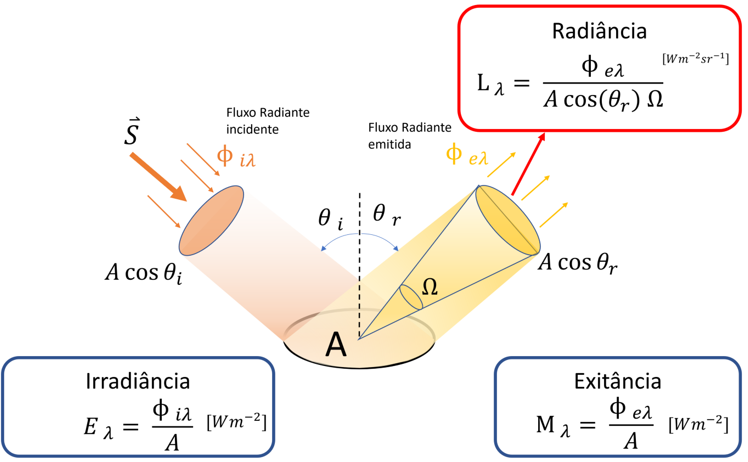
\includegraphics[width=0.75\linewidth]{images/remote_detection_principles.png}

    \caption{Geometric definitions of the fundamental radiometric primitives. The diagram illustrates the distinction between the hemispherical fluxes of Irradiance ($E_\lambda$) and Exitance ($M_\lambda$), normalized by surface area $A$, versus the directional quantity of Radiance ($L_\lambda$), normalized by projected area $A \cos \theta_r$ and solid angle $\Omega$. Effects of atmospheric transmittance and path radiance are implicitly assumed in the propagation. (TODO:Update with new variable and add satellites, athmosphere etc.}

    \label{fig:remote_sense_radiometric_primitives}

\end{figure}



Consider the study domain $\mathcal{D}$ with a region target $\mathcal{R} \in \mathcal{F}_\oplus$ observed by a satellite as represented in Fig. \ref{fig:remote_sense_radiometric_primitives}. An elementary plane surface patch $S_j$, with $S_j \in \mathcal{R}$, has its area $A$ irradiated by electromagnetic radiation from the pointing vector $\vec{S}$ at an incidence angle $\theta_i$ with respect to the surface normal. Let $Q_{\lambda}$ be the radiant energy in a narrow spectral interval around wavelength $\lambda$ that crosses area $A$ within time $\Delta t$. The corresponding \textbf{spectral radiant flux} is

\begin{equation}

\phi_{\lambda} \;=\; \frac{Q_{\lambda}}{\Delta t}\quad [\mathrm{W}]\,.

\label{eq:spectral_radiant_flux}

\end{equation}

The incident flux per unit area is the \textbf{spectral irradiance} $E_{\lambda}$,

\begin{equation}

E_{\lambda} \;=\; \frac{\phi_{\lambda,i}}{A}\quad [\mathrm{W\,m^{-2}}] \,,

\label{eq:spectral_irradiance}

\end{equation}

while the flux \emph{leaving} the surface per unit area is the \textbf{spectral exitance} $M_{\lambda}$,

\begin{equation}

M_{\lambda} \;=\; \frac{\phi_{\lambda,e}}{A}\quad [\mathrm{W\,m^{-2}}] \;.

\label{eq:spectral_exitance}

\end{equation}

Radiance introduces directionality. The spacecraft detector at point $P_{sat}$, $P_{sat}(x^\mu)\footnote{We adopt General Relativity index notation (e.g., Carroll, \emph{Spacetime and Geometry}) for compactness, independent of the relativistic framework. Greek indices run $\mu=0,\dots,3$ (spacetime) and Latin indices $i=1,\dots,3$ (space). Thus, $x^\mu = (x^0, x^1, x^2, x^3) = (ct, x, y, z)$, with $t \in \mathcal{T}$ a temporal domain.} \in \mathcal{F}_{J2000}$, observes surface $S_j$ at the centralized target point $P_{target}$, $P_{target}(x^\nu) \in \mathcal{F}_{J2000}$, connected via the Line-of-Sight vector $\vec{r}_{LoS} = P_{target} - P_{sat}$. This instrument has a viewing direction that makes an angle $\theta_r$ with respect to the surface normal. The satellite detector, with an effective sensitive area $A_D$, collects the emitted radiant flux $\phi_{\lambda,e}$ over the solid angle $\Omega$. The \textbf{spectral radiance} measured by the detector is

\begin{equation}

L_{\lambda} \;=\; \frac{\phi_{\lambda,e}}{A\,\cos\theta_r\,\Omega}\quad [\mathrm{W\,m^{-2}\,sr^{-1}\,\mu m^{-1}}] \,.

\end{equation}



\subsubsection{From Radiance to Digital Number (DN)}

Satellites do not record radiance directly. Detectors convert incident photons into electric charge, which is quantized by an Analog-to-Digital Converter (ADC) into a discrete \textbf{Digital Number (DN)}. Recovering physical radiance requires radiometric calibration. While full sensor characterization is outside this work's scope, the process is generally approximated by a linear model for a spectral band $b$:

\begin{equation}

\mathrm{DN}_b \;\approx\; g_b\,L_{b,\mathrm{toa}} + o_b\,,

\end{equation}

where $g_b$ is the gain, $o_b$ the offset, and $L_{b,\mathrm{toa}}$ is the \textbf{Top-of-Atmosphere (TOA) band radiance}. Inverting this relation is the prerequisite for any physical interpretation of the fire scene.



\subsubsection{Radiance as a composition of reflective and emissive processes}

In a rigorous physical framework, spectral radiance is the superposition of multiple mechanisms: reflection, thermal emission, and secondary effects such as inelastic scattering (e.g., Raman) and luminescence. However, for the energy magnitudes involved in wildfire remote sensing, secondary quantum effects are negligible compared with solar reflection and thermal blackbody emission. Therefore, we approximate the surface radiance as a sum of two dominant components:

\begin{equation}

L_{\lambda,\mathrm{surf}} \;\approx\; L_{\lambda,\mathrm{refl}} + L_{\lambda,\mathrm{therm}}\,.

\end{equation}

The reflected component is driven by solar illumination and surface bidirectional reflectance (BRDF), while the thermal component is governed by temperature and emissivity (Planck's Law). A practical first-order forward model for what the satellite measures at TOA is:

\begin{equation}

L_{\lambda,\mathrm{toa}} \;=\; \tau_{\lambda}\,L_{\lambda,\mathrm{surf}} \; +\; L_{\lambda,\mathrm{path}}\,.

\end{equation}

Here $\tau_{\lambda}$ is the atmospheric transmittance along the line of sight and $L_{\lambda,\mathrm{path}}$ is the path radiance (scattering and atmospheric emission) added between the ground and the sensor. Transmittance is the superposition of terms:

\begin{equation}

\tau_{\lambda} \;\approx\; \tau_{\lambda,\mathrm{gas}}\,\tau_{\lambda,\mathrm{aer}}\,\tau_{\lambda,\mathrm{smoke}}\,\tau_{\lambda,\mathrm{cloud}}\,,

\label{eq:tranmitance_atm}

\end{equation}

where the last two terms highlight how \textbf{smoke} and \textbf{cloud} can severely attenuate the signal. These terms are treated in Sec.~\ref{321-atmospheric-transmittance-and-attenuation} in the context of observability constraints.

\paragraph{The limit of Reflectance products for Fire detection.}

Many Earth Observation products are reported as a radiance-normalized surface reflectance ($\rho_\lambda$), intuitively defined as the ratio of exiting flux to incoming flux:

\begin{equation}

\rho_{\lambda} \;= \frac{M_\lambda}{E_\lambda} \;\approx\; \frac{\pi\,L_{\lambda,\mathrm{surf}}}{E_{\lambda,\mathrm{down}}\,\cos\theta_i}\quad (\text{Lambertian approx.})\,.

\end{equation}

For standard land cover, this approximation holds because the upwelling radiance is dominated by reflection ($L_{\lambda,\mathrm{surf}} \approx L_{\lambda,\mathrm{refl}}$). However, active fires break this intuition. For a fire pixel, the surface is not only reflecting sunlight but is also \emph{actively emitting} intense thermal radiation ($L_{\lambda,\mathrm{therm}}$). 



If one were to apply the standard reflectance formulation and calibration with sun light as reference to a fire pixel, the additional term $L_{\lambda,\mathrm{therm}}$ would result in a mathematically valid but physically misleading "reflectance" value (often $> 1.0$). Consequently, fire characterization cannot rely on passive reflective metrics. Instead, it requires isolating the thermal excess to quantify the energy release by the combustion of the material. This necessitates a dedicated metric: \textbf{Fire Radiative Power (FRP)}. 



FRP provides a direct quantitative link to the amount of biomass consumed (combustion rate) and the intensity of the fire front. 



\section{The Fire Itself: Physics of the Radiative Signature}

\label{31-the-fire-itself-physics-of-the-radiative-signature}



This chapter establishes the physical foundation linking the thermal emission of a wildfire to the digital signal received 

\subsection{Physical Limit: Atmospheric Attenuation}
\label{subsec:atmospheric_limit}
As discussed in the Radiance Chapter, the infrared signal is modulated by the atmospheric transmittance $\tau_\lambda$ (Eq. \ref{eq:tranmitance_atm}). Factors such as clouds, smoke aerosols, and water vapor significantly attenuate the signal.

Observations at low elevation angles $\varepsilon$ (near the horizon) traverse a much thicker atmospheric layer compared to the Zenith path, drastically degrading the Signal-to-Noise Ratio (SNR). The path length through the atmosphere scales with $\approx 1/\sin(\varepsilon)$. 

To mitigate these effects without performing complex real-time radiative transfer modelling, we impose a strict geometric constraint. We define the operational limits: the \textbf{Minimum Elevation Angle} $\varepsilon_{min} = 15^\circ$, \inlineReq{R29}, and \textbf{Maximium Athmospheric grazing angle} $\theta{\text{atm max}}=65^\circ$, \inlineReq{R30}. 

This threshold acts as a proxy for signal quality, filtering out observations where transmittance is likely to be dominated by scattering and absorption.

\subsection{Geometric Access Windows}
Based on the physical limit defined above, we construct two geometric volumes that define the valid observation space, as illustrated in Fig. \ref{fig:access_nominal_and_limit}.

\begin{figure}[H]
    \centering
    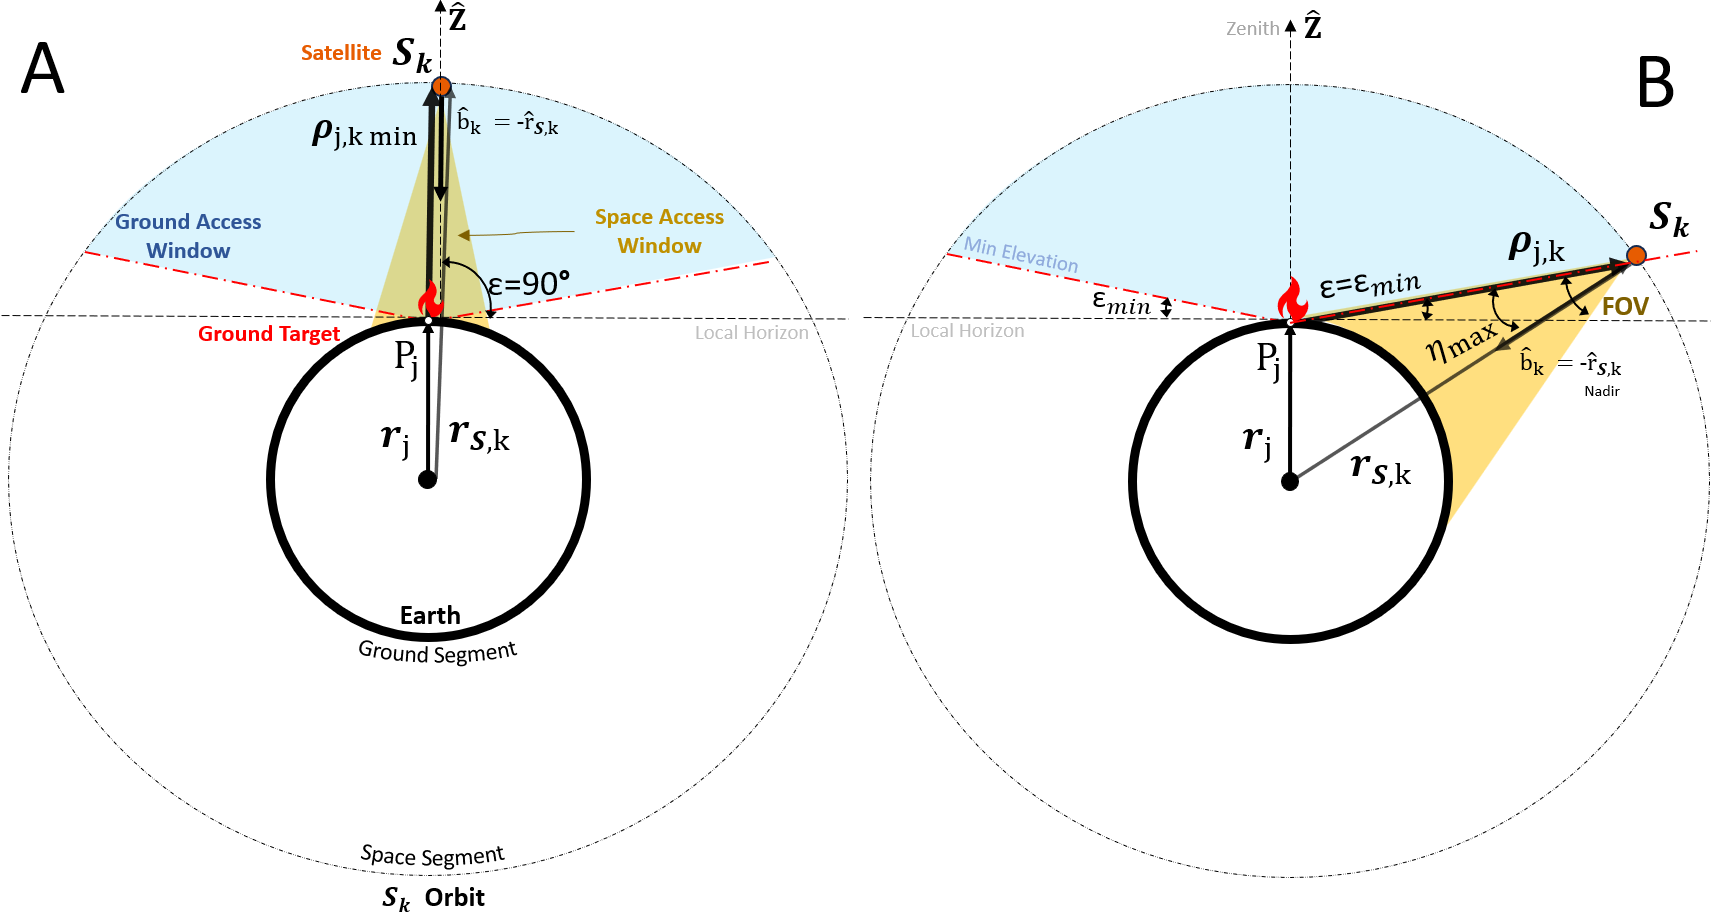
\includegraphics[width=1\linewidth]{images/access_nominal_and_limit.png}
    \caption{Geometric definition of the Observation Constraints. The valid detection volume is formed by the intersection of the Ground Access Window (Orange) and the Space Access Window (Blue). A) Highlights the Nominal Zenith case (best quality) where ground resolution GSD is calculated. B) Visibility limit configuratrion, edge of the coverage where Ground \& Space Access windows meet ($\epsilon_{min}$ and $\eta_{max}$).}
    \label{fig:access_nominal_and_limit}
\end{figure}

\subsection{Ground Access Window ($\mathcal{W}_{ground}$)}
The Ground Access Window $\mathcal{W}_{ground,j}$ represents the volume of the local sky physically visible and useful to the target point $P_j$. While a target theoretically has a $180^{\circ}$ view of the sky (from horizon to horizon), practical observation is limited by terrain geometric masking and atmospheric attenuation.

We define the constraint using the \textbf{Elevation Angle $\varepsilon$}, measured from the local horizon to the satellite. To ensure valid data retrieval, the satellite must be above a minimum elevation threshold:
\begin{equation}
    \mathcal{W}_{ground,j} = \{ \text{Visible} \mid \varepsilon \geq \varepsilon_{min} \}
\end{equation}
For this mission analysis, as discussed, we set the requirement to $\varepsilon_{min} = 15^{\circ}$. Below this angle, the path length through the atmosphere increases drastically, degrading the signal-to-noise ratio and geometric accuracy.

\subsection{Space Access Window ($\mathcal{W}_{space}$)}
The Space Access Window represents the conical volume observable by the spacecraft $S_k$. This volume encloses all potential instrument architectures (e.g., push-broom scanners, matrix cameras) and is defined relative to the satellite's Sensor Boresight Vector $\hat{\mathbf{b}}_k$, which nominally points toward the geodetic Nadir.

We define the constraint using the \textbf{Off-Nadir Angle $\eta$}, measured from the boresight vector $\hat{\mathbf{b}}_k$ to the the Relative Position Vector $\vec{\rho}_{j,k}$ between ground target $P_j$ and the satellite $S_k$. The limit is determined by the maximum reachable angle of the spacecraft optical system:
\begin{equation}
    \mathcal{W}_{space} = \{ \text{Visible} \mid \eta \leq \eta_{max} \}
\end{equation}
For a standard Earth-observation missions (LEO-MEO), achieving the good quality optical signal typically demands a maximum off-nadir view of $\eta_{max} = \theta{\text{atm max}} \approx 65^{\circ}$, \inlineReq{R31}. This cone defines the max Full Field of View for the satellites, \inlineReq{R32}.
\begin{equation}
    FOV = 2  \eta_{max} = 130^\circ; 
\end{equation}
\subsection{The Visibility Condition}
Consequently, a fire event at $P_j$ is only detected when the satellite enters the intersection of these two windows as shown in Fig \ref{fig:access_nominal_and_limit}-B. The geometric requirement for observation is the simultaneous satisfaction of both access windows angular constraints\inlineReq{R33}:

\begin{equation}
    \text{Observation Link} \ \mathcal{L}_{j,k} \iff Visible
    \begin{cases} 
        \varepsilon \geq 15^{\circ} & \text{(Ground access: clear sky horizon)} \\
        \eta \leq 65^{\circ} & \text{(Space access : sensor athmospheic gazing limit)}
    \end{cases}
\end{equation}

\subsection{Optical Quality: Ground Sample Distance (GSD)}
\label{optical-quality}
The spatial resolution of the detected fire is governed by the \textbf{Ground Sample Distance (GSD)}. For this constellation design analysis we have the spacecraft at the nadir configuration as shown in Fig \ref{fig:access_nominal_and_limit}-A. On this observation setting, we utilize the first-order paraxial approximation calculated at nadir, \inlineReq{R34}. The GSD is deffined in function of the satellite altitude $h(t) = \|  \vec{\rho}_{j,k}  \| - \vec{r}_j$:
\begin{equation}
    \text{GSD}(t) \approx \frac{p \cdot h[n]}{f}
\end{equation}
where $p$ is the detector pixel pitch and $f$ is the effective focal length. Athmospheric effects is not taking in consideration. 

\paragraph{Simulation Parameters:}
For the specific instrument modeled in this thesis, we assume the following optical characteristics:
\begin{itemize}
    \item Pixel Pitch: $p = $ [(TODO:TBD)]
    \item Focal Length: $f = $ [(TODO:TBD)]

    \chapter{Fundamentals of Satellite Constellation
Design}\label{chapter-7-fundamentals-of-satellite-constellation-design}

Observation: This chapter will have the structure detailed during the
development.

\begin{quote}
\textbf{Writing Guide \& Methodological Focus:}

\begin{itemize}
\item
  \textbf{Objective:} To provide the reader with the necessary
  theoretical knowledge to understand the design and analysis.
\item
  \textbf{Method:} Present the core concepts of orbital mechanics and
  constellation design clearly and concisely.
\item
  \textbf{Checkpoint:} Does this chapter give the reader all the
  foundational knowledge they need to understand the simulation work in
  Chapter 8?
\end{itemize}
\end{quote}

\section{Constellation Observation Formalism Introduction}
\label{sec:Constellation_observation_form}
%Improve intro reflection full section
We have previously defined the study domains $\mathcal{D}$ on the Earth's surface. However, for a fire event to be detected, it must fall within the observable coverage domain of the satellite constellation $\mathcal{D_{Cover}}$.  

\subsection{Constellation Definition and State Space}
The satellite constellation is defined as a set of $N$ discrete spacecraft nodes:
\begin{equation}
    \mathcal{C}_{sat} = \{ S_k \}_{k=1}^{N}
\end{equation}
Each satellite $S_k$ is uniquely defined by its \textbf{Orbital State Element} $\vec{A}_k$:
\begin{equation}
    S_{k} \equiv \vec{A}_k
\end{equation}
This vector encapsulates the state-space parameters required to propagate the spacecraft's trajectory. The detailed definition of $\vec{A}_k$ is provided in the Methodology section, as it depends on the specific orbit type.


\subsection{Single-Satellite Sensor Visibilty Toward a Ground Target}
This section defines the geometric boundaries and optical constraints that govern the visibility link between a ground target and a spacecraft sensor. The revisit time $t_{rev \to P_j}$ of a satellites $\mathcal{S}_{k}$ over a ground point target $P_{j}$ is fundamentally limited by the geometric constraints of the spacecraft sensor relative to the ground location. To quantify these constraints, such as whether a target is above the local horizon or within the sensor's field of view, we must define a coordinate frame system centered on the observer's location at ellipsoid surface $\mathcal{E_\oplus}$.  The detailled deffinition of such local frame, the satellite and ground trajectory is done in section 

\paragraph{Satellite Position Trajectory:}
To analyze geometric of the sensor to a target, we first define the trajectories of the spacecraft and the ground targets as time-dependent mappings on the inertial manifold $\mathcal{M}$, as defined in eq. \ref{eq:manifold}. Than, we define the $k$-th satellite $S_k$ as a point mass moving in the inertial frame. Its orbital position with respect to Earth's center of mass $O_{\oplus}$ is defined by the position vector function $\vec{r}_{s,k}$:
\begin{equation}
    \vec{r}_{s,k} : \mathcal{T}_{sim} \to \mathcal{M}, \quad t \mapsto \overrightarrow{r_{s,k}}(t) = \overrightarrow{O_{\oplus}S_{k}}(t)
\end{equation}
\paragraph{Ground Target Trajectory:}
The ground target $P_j$ is fixed to the surface of the WGS84 Reference Ellipsoid $\mathcal{E}_\oplus$. However, due to the Earth's rotation, $P_j$ describes a trajectory in the inertial frame $\mathcal{F}_{J2000}$. We define this motion as the vector function $\vec{r}_j$:
\begin{equation}
    \vec{r}_{j} : \mathcal{T}_{sim} \to \mathcal{M}, \quad t \mapsto \overrightarrow{r_j}(t) = \overrightarrow{O_{\oplus}P_{j}}(t)
\end{equation}
\subsubsection{Topocentric Horizon Coordinate System (SEZ)}
The Topocentric Horizon Coordinate System $\mathcal{F}_{SEZ}$ is the standard frame for defining "look angles" between a ground site and a satellite. We adopt the deffitintion of $\mathcal{F}_{SEZ}$ as done by Vallado\cite{mcclain2001fundamentals}. This frame is also know as $\mathcal{F}_{AltAz}$ because it measure the altitude, also know as elevation $\epsilon$,  and azimuth $\beta$ as shown in Fig. \ref{fig:sez_frame}, this system rotates with the site location $P_{k}$.

\begin{figure}[H]
    \centering
    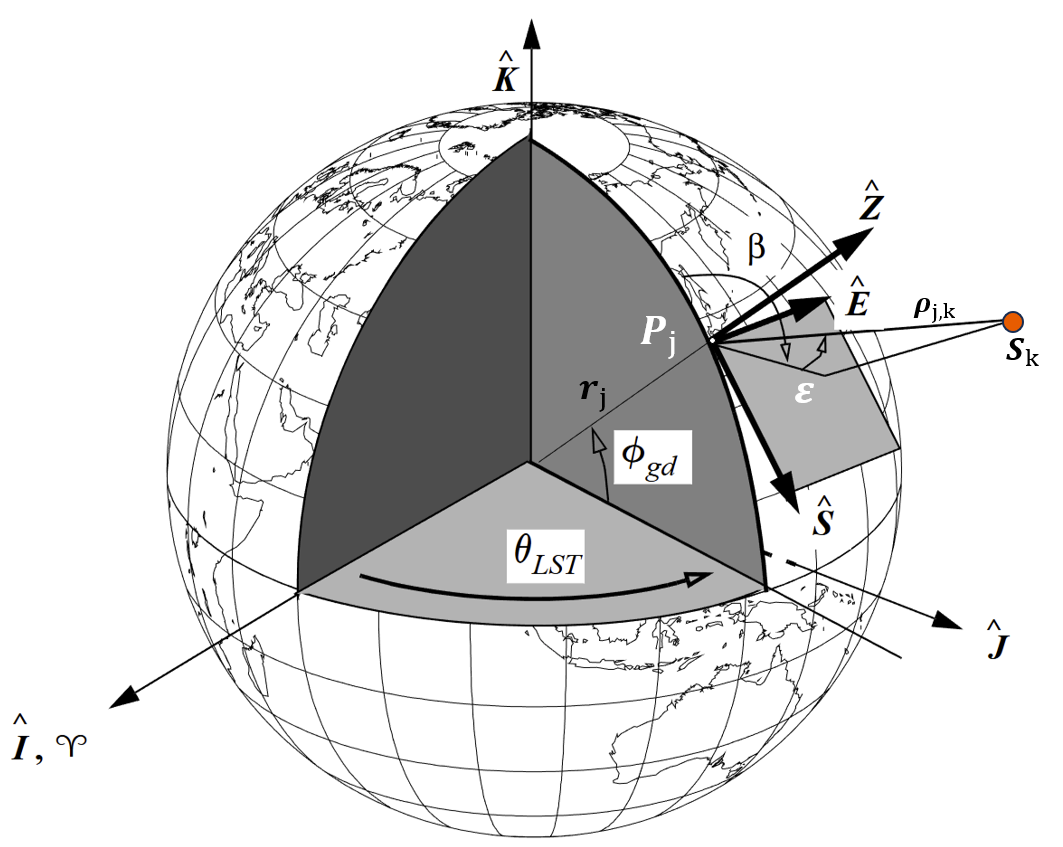
\includegraphics[width=0.6\linewidth]{images/Topocentric_Horizon_Coordinate_System_SEZ.png}
    \caption{\footnotesize{The Topocentric Horizon Coordinate System  $\mathcal{F}_{SEZ}$, "South, East, Zenith frame", or $\mathcal{F}_{AltAz}$. The frame originates at the site location $P_k$ on the Earth's elipsoid $\mathcal{E_\oplus}$. The fundamental plane is the local horizon. The $\hat{S}$ axis points South, the $\hat{E}$ axis points East, and the $\hat{Z}$ axis (Zenith) points radially outward along the local vertical. $\mathcal{F}_{SEZ}$ defines the observation geometry: Azimuth $\beta$ measured clockwise from North, and Elevation $\epsilon$ measured from the horizon plane up to the vector $\rho_{j,k}$ measuring the relative distance between satellite $S_k$ and the ground target $P_j$ .}}
    \label{fig:sez_frame}
\end{figure}
This planetary mobile local frame is is defined by the orthonormal basis $\mathcal{B}_{SEZ} = \{ \hat{\mathbf{s}}, \hat{\mathbf{e}}, \hat{\mathbf{z}} \}$ centered at the target $P_j$, $\mathcal{F}_{SEZ} \equiv  \{ P_{j};\hat{\mathbf{s}}, \hat{\mathbf{e}}, \hat{\mathbf{z}} \}$.  The unit vectors are defined as: $\hat{\boldsymbol{s}}$ (South) along the local meridian, $\hat{\boldsymbol{e}}$ (East) along the local parallel, and $\hat{\boldsymbol{z}}$ (Zenith) along the local vertical

\paragraph{Line-of-Sight (LOS) Vector:}
The relative geometry is governed by the vector connecting the ground target $P_j$ to the satellite $S_k$. We construct this \textbf{Line-of-Sight Vector} $\vec{\rho}_{j,k}$ via the vector subtraction map:
\begin{equation}
    \vec{\rho}_{j,k} : \mathcal{T}_{sim} \to \mathcal{M}, \quad t \mapsto \overrightarrow{\rho_{j,k}}(t) = \overrightarrow{P_{j}S_{k}}(t) = \overrightarrow{r_{s,k}}(t) - \overrightarrow{r_{j}}(t)
\end{equation}

This vector is projected onto the local basis $\mathcal{B}_{SEZ}$ as:
\begin{equation}
    \vec{\rho}_{j,k} = \rho_s \hat{\mathbf{s}} + \rho_e \hat{\mathbf{e}} + \rho_z \hat{\mathbf{z}}
\end{equation}
%%
\paragraph{Relative Position Vector ($\vec{\rho}_{j,k}$):}
The geometry is commanded by the relative displacement between the ground target $P_j$ and the satellite $S_k$. We define the \textbf{Relative Position Vector}  $\vec{\rho}_{j,k}$ via the vector subtraction map:
\begin{equation}
    \vec{\rho}_{j,k} : \mathcal{T}_{sim} \to \mathcal{M}, \quad t \mapsto \vec{\rho}_{j,k}(t) = \overrightarrow{P_{j}S_{k}}(t) = \overrightarrow{r_{s,k}}(t) - \overrightarrow{r_{j}}(t)
\end{equation}
This vector represents the physical distance and direction from the target to the satellite, independent of where the satellite is facing. It is projected onto the local basis $\mathcal{B}_{SEZ}$ as:
\begin{equation}
    \vec{\rho}_{j,k} = \rho_s \hat{\mathbf{s}} + \rho_e \hat{\mathbf{e}} + \rho_z \hat{\mathbf{z}}
\end{equation}
\paragraph{Sensor Boresight Vector ($\hat{\mathbf{b}}_k$):}
Distinct from the relative position, the satellite $S_k$ observation capability depends on its attitude and sensor direction. We define the Sensor Boresight Vector (or Line-of-Sight direction) as the unit vector $\mathbf{b}_{k}$  representing the optical axis of the instrument in the inertial frame:
\begin{equation}
    \hat{\mathbf{b}}_{k} : \mathcal{T}_{sim} \to \mathcal{M}, \quad t \mapsto \hat{\mathbf{b}}_{k}(t) = \mathbf{A}(t) \cdot \hat{\mathbf{b}}_{body}
\end{equation}
where, for $S_k$, $\mathbf{A}(t)$ is the attitude rotation matrix and $\hat{\mathbf{b}}_{body}$ is the fixed sensor axis in the satellite body frame.

\paragraph{Look Angles Definition:}
From these components, we define the look angles as the mapping $\Lambda_{look}: \mathbb{R}^3 \to \mathbb{R}^2$:

\begin{enumerate}
    \item \textbf{Elevation ($\varepsilon$):} The angular height above the local horizon plane. It is derived from the angle between the local zenith $\hat{\mathbf{z}}$ (aligned with $\hat{\boldsymbol{r}}_{j}$ for a spherical approximation) and the relative vector:    \begin{equation}
        \epsilon_{k,j} = \sin^{-1}\left( \frac{\vec{\rho}_{j,k} \cdot \hat{\mathbf{z}}}{\| \vec{\rho}_{j,k} \|} \right), \quad \varepsilon \in \left[ -\frac{\pi}{2}, \frac{\pi}{2} \right]
    \end{equation}
    A positive elevation ($\varepsilon > 0$) indicates that the satellite is above the local geometric horizon and may be able to observe $P_j$, depending on the spacecraft's sensor field of view, line-of-sight orientation, and atmospheric transmission. 
    \item \textbf{Azimuth ($\beta$):} The orientation angle measured clockwise from North ($-\hat{\mathbf{s}}$) to the projection of the satellite vector on the horizon plane.
\begin{equation}
        \beta_{k,j} = \operatorname{atan2}(\rho_e, -\rho_s), \quad \beta \in [0, 2\pi)
    \end{equation}
    where $\operatorname{atan2}(y, x)$ is the multi-valued inverse tangent function used to resolve quadrant ambiguity.
\end{enumerate}

\section{Observational Access}
\label{sec:observational_access}
To formally characterize the observation geometry, we adapt the constellation observation visibility framework established by Lee et al. \cite{lee_satellite_2020}. We introduced the sensor constraints as a condition for visibility.
For a valid observation to occur, the geometric link must satisfy constraints from two distinct reference frames: the target's local horizon (Ground Segment) and the satellite's instrument orientation (Space Segment). As illustrated in Figure \ref{fig:access_window_configs}, visibility is only achieved when the Line-of-Sight (LOS) vector falls within the intersection of these two independent access volumes.

\begin{figure}[H]
    \centering
    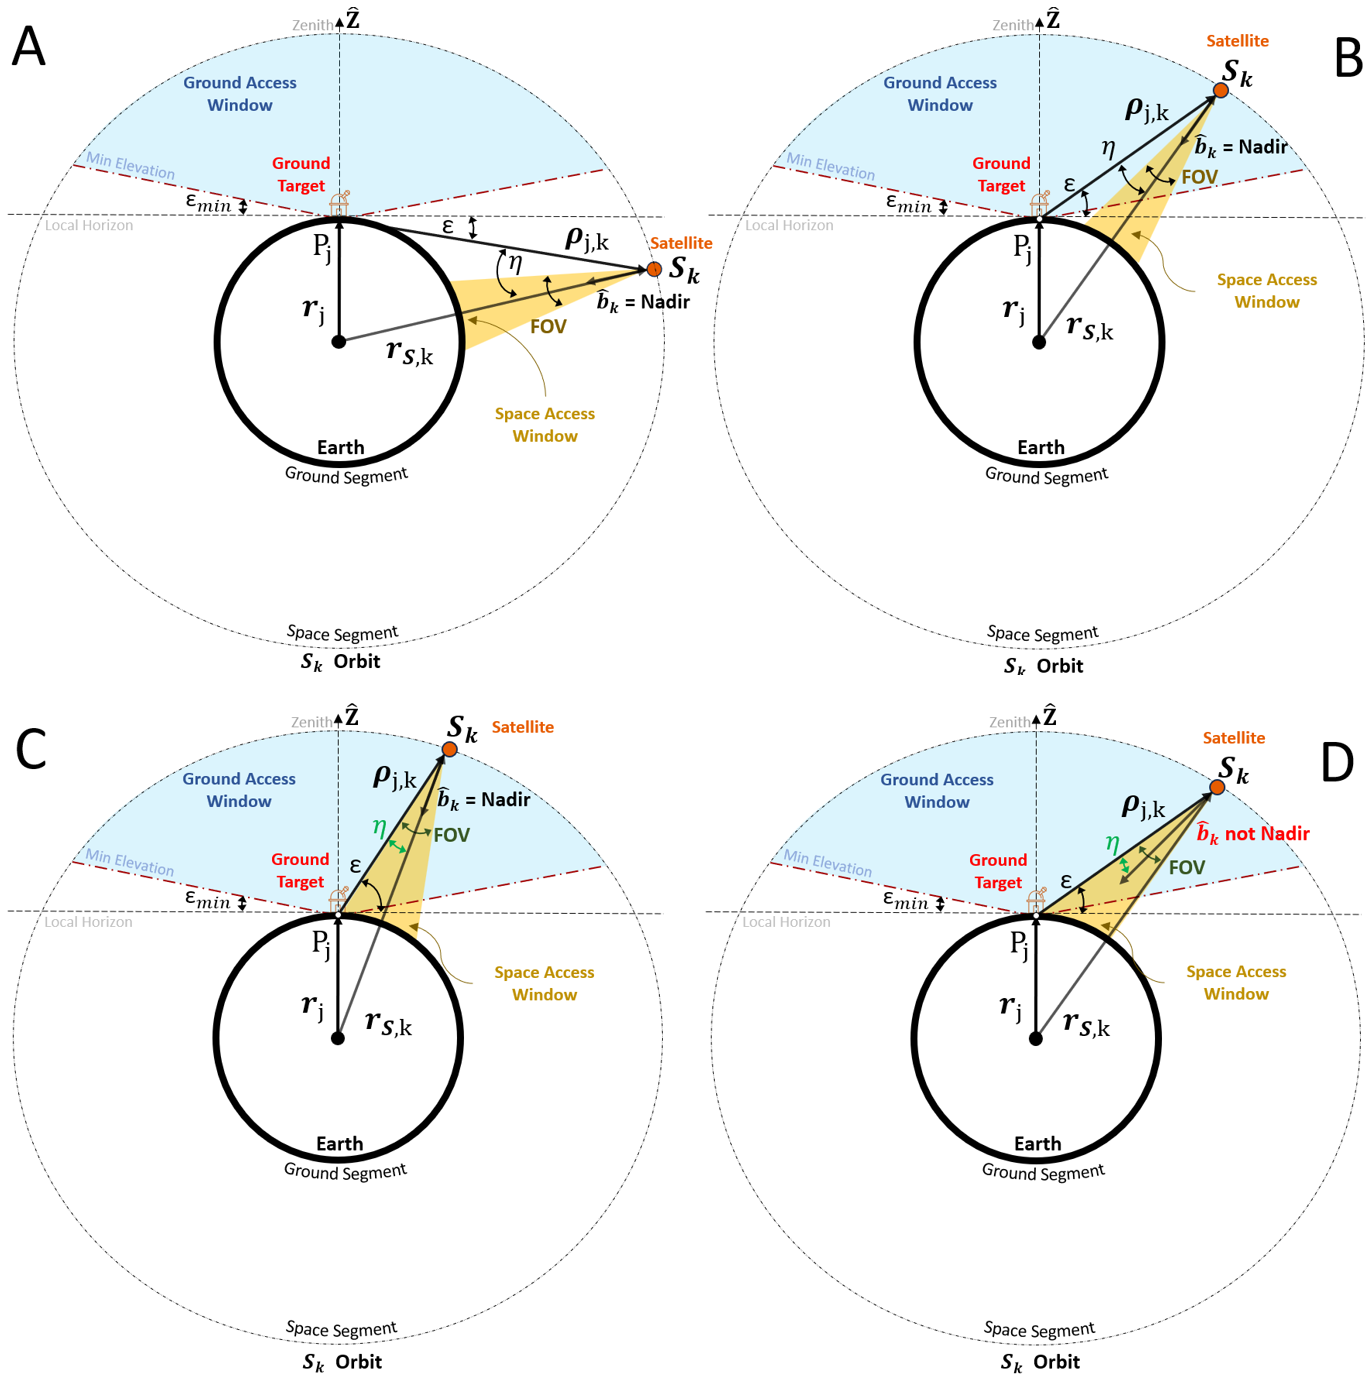
\includegraphics[width=1\linewidth]{images/acess_window_configs.png}
    \caption{Observational Access Windows configuration. The figure illustrates the interaction between the \textbf{Ground Access Window} (blue cone, defined by tange point $P_j$ and $\epsilon_{min}$) and the \textbf{Space Access Window} (yellow cone, defined by the sensor direction $\hat{b}_k, FOV, $$\eta_{max}$).
    \textbf{(A)} No access: satellite is below the local horizon.
    \textbf{(B)} Ground access, no space access: satellite is above the horizon but with FOV outside $P_j$, or $\eta > FOV$.
    \textbf{(C)} Space \& ground access: satellite see ground $P_j$, ($\epsilon > \epsilon_{min}$) \& ($\eta < FOV$).
    \textbf{(D)} Space \& ground access with pointing out of nadir: $S_k$ uses point mechanism to have valid angular view from $P_j$ $(\theta \leq FOV)$.} (TODO:Update reducing redudant info)
    \label{fig:access_window_configs}
\end{figure}

\subsection{Ground Segment Access Window ($\mathcal{W}_{ground}$)}
From the perspective of the target $P_j$, $P_j \in \mathcal{F}_{SEZ}$, the satellite $S_k$ must appear within a specific volume of the local sky to ensure a clear signal path. We define the Ground Access Window as the subset in the the Topocentric frame $\mathcal{F}_{SEZ}$ where the elevation angle exceeds the minimum operational threshold $\epsilon_{min}$ (imposed by terrain geometric masking and atmospheric attenuation).

Mathematically, this domain is defined by the condition on the relative position vector $\vec{\rho}_{j,k}$ with the spacecraft:
\begin{equation}
    \mathcal{W}_{ground_{j,k}}(t) = \{ \vec{\rho}_{j,k} \in \mathcal{M} \mid \epsilon(\vec{\rho}_{j,k}) \geq \epsilon_{min} \}
\end{equation}
where $\epsilon(\vec{\rho}_{j,k})$ is the elevation calculation defined in the previous section.

\subsection{Space Segment Access Window ($\mathcal{W}_{space}$)}
From the perspective of the satellite $S_k$, the target $P_j$ must lie within the instrument's Field of View (FOV). We define the \textbf{Space Access Window} (or Sensor Cone) based on the instrument's half-cone angle $\eta_{max}$ (FOV limit) relative to the instantaneous boresight vector $\hat{\mathbf{b}}_k(t)$.

The \textbf{Off-Nadir Angle} $\eta_{k,j}$ is defined as the angle between the sensor boresight and the direction to the target (which is $-\vec{\rho}_{j,k}$ in the satellite frame):
\begin{equation}
    \eta_{k,j}(t) = \arccos\left( \frac{-\vec{\rho}_{j,k}(t) \cdot \hat{\mathbf{b}}_{k}(t)}{\| \vec{\rho}_{j,k}(t) \|} \right)
\end{equation}
The Space Access Window is therefore the volume where this angle satisfies the optical limit:
\begin{equation}
    \mathcal{W}_{space_{j,k}}(t) = \{ \vec{\rho} \in \mathcal{M} \mid \eta(\vec{\rho}_{j,k}, \hat{\mathbf{b}}_k(t)) \leq \eta_{max} \}
\end{equation}
\subsection{Total Visibility Condition}
A valid observation event $E_{obs}$ occurs at time $t$ if and only if the Line-of-Sight vector exists within the intersection of both domains. Formally:
\begin{equation}
    \text{Visible}(t) \iff \vec{\rho}_{j,k}(t) \in \left( \mathcal{W}_{ground_{j,k}}(t) \cap \mathcal{W}_{space_{j,k}}(t) \right)
\end{equation}
This is equivalent to the simultaneous satisfaction of the two scalar inequalities:
\begin{equation}
    \text{Observation Link} \ \mathcal{L}_{j,k}(t) \iff Visible
    \begin{cases} 
        \epsilon_{k,j}(t) \geq \epsilon_{min} =15^{\circ} & \text{(Ground Access Condition)} \\
        \eta_{k,j}(t) \leq \eta_{max} = 65^{\circ} & \text{(Space Access Condition)}
    \end{cases}
\end{equation}

